\section{Evaluation}

In the last chapter, we presented an implementation of the presented methods to infer time, size and cost bounds.
This chapter evaluates this implementation against other methods.

For this purpose, two different approaches are used.
First, some selected examples are presented, where the benefit of the presented method in contrast to method of the original KoAT \cite{koat} is shown.
Second, the implementation is evaluated on an example set of programs, defined and used by comparable tools with the same objective of inferring time bounds for integer programs.

\subsection{Evaluating selected examples}

In this section, we use two selected examples to compare the results of the new method with the results of the original KoAT \cite{koat}.
This selection is chosen to show the benefits of the new method and is by no means representative.
Nevertheless it is able to show the potentials of the new method.

\todo{Activate picture}{}
\iffalse\begin{figure}
  \centering
  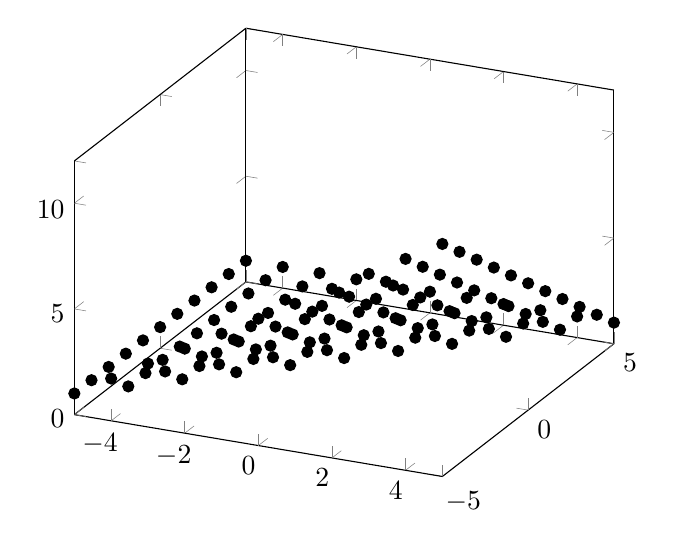
\begin{tikzpicture}
    \begin{axis}
      \addplot3 [
        unbounded coords=jump,
        mesh,
        shader=interp,
        samples at={-5,...,5},
        samples y={11},
        only marks,
      ] {1+max(x-y,0)};
    \end{axis}
  \end{tikzpicture}
  \hfil
  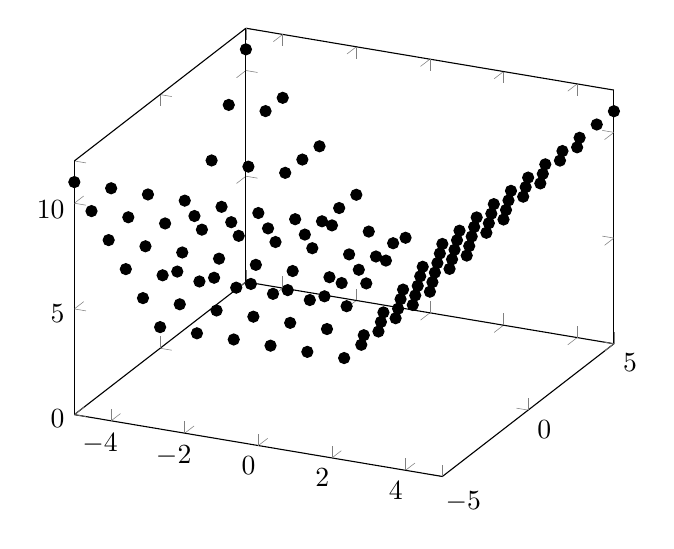
\begin{tikzpicture}
    \begin{axis}
      \addplot3 [
        unbounded coords=jump,
        mesh,
        shader=interp,
        samples at={-5,...,5},
        samples y={11},
        only marks,
      ] {1+abs(max(x,-y))+abs(max(x,-y))};
    \end{axis}
  \end{tikzpicture}
  \caption{Evaluation of the motivational example}
  \label{fig:motivational_evaluation}
\end{figure}
\fi

\subsection{Evaluating an example set}

In this section, the presented implementation is evaluated on an example set, which is a collection of examples introduced by other tools.
The main focus is a comparison with the method of the original KoAT paper \cite{koat}.
Besides that we compare the implementation to the tool CoFloCo \cite{cofloco3}.
For both KoAT and CoFloCo we use the latest development version available at the time of this thesis.

For the comparison of the results, it is necessary to project the resulting bounds in $\BoundSet(\PVSet)$ to their asymptotic complexity class.
The following definition introduces a projection, such that for every bound $b \in \BoundSet(\PVSet)$ the resulting asymptotic complexity $\complexity(b)$ is a valid overapproximation of the actual complexity.

\begin{definition}[Approximation of the asymptotic complexity]
  Let $\BoundSet(\VSet)$ be a set of bounds over the variables $\VSet$.
  Let $\landau$ be the landau symbol for asymptotic complexity.
  Then, $\complexity$ is a function which assigns each bound an overapproximation of its asymptotic complexity.
  \[ \complexity(\infty) = \landau(\infty) \text{ for } \infty \in \BoundSet(\VSet) \]
  \[ \complexity(k) = \landau(1) \text{ for all } k \in \mathbb{N} \subset \BoundSet(\VSet) \] 
  \[ \complexity(v) = \landau(n) \text{ for all } v \in \VSet \subset \BoundSet(\VSet) \] 
  \[ \complexity(-b) = \complexity(b) \text{ for all } b \in \BoundSet(\VSet) \] 
  \[ \complexity(b_1 + b_2) = \landau(\complexity(b_1) + \complexity(b_2)) \text{ for all } b_1, b_2 \in \BoundSet(\VSet) \] 
  \[ \complexity(b_1 \cdot b_2) = \landau(\complexity(b_1) \cdot \complexity(b_2)) \text{ for all } b_1, b_2 \in \BoundSet(\VSet) \] 
  \[ \complexity(\max(b_1, b_2)) = \landau(\max(\complexity(b_1), \complexity(b_2))) \text{ for all } b_1, b_2 \in \BoundSet(\VSet) \]
  \[ \complexity(k^b) = k^{\complexity(b)} \text{ for all } k \in \mathbb{N} \subset \BoundSet(\VSet), b \in \BoundSet(\VSet) \]  
\end{definition}

Note that this definition projects a bound $x-x$ to a complexity $\complexity(x-x) = \landau(n)$.
As already mentioned, the implementation is able to simplify such bounds to an equivalent bound $0$.
Therefore the better, but still valid complexity $\complexity(0) = \landau(1)$ is determined.
Nevertheless the implementation is not able to simplify every bound $b$ to an equivalent bound $b'$ with a complexity $\complexity(b')$ better than $complexity(b)$, although such a bound $b'$ exists.
Such a simplification algorithm has high performance costs for the implementation.
Therefore, the implemented simplification algorithm does in general not support the simplification of bounds, where it is necessary to analyze multiple levels of operators like $3 \cdot x^2-(x \cdot x+2 \cdot x^2)$.
Thus, an optimized simplification algorithm might yield better evaluation results without a change to the presented method.

For the parallel execution of the examples, we use the GNU tool 'parallel' \cite{gnuparallel}.
This way, the evaluation of all examples takes \todo{Insert time}{x} seconds with an average of \todo{Insert time}{x} seconds on an Intel i7 processor with four cores.
Therefore, the performance of the new implementation is comparable to other tools of the same domain.

\begin{table}
  \begin{center}
    \label{tab:evaluation}
    \begin{tabular}{l|c|c|c|c|c|c|c|c|c|c|c}
      Method & $\landau(1)$ & $\landau(n \log n)$ & $\landau(n)$ & $\landau(n^2)$ & $\landau(n^3)$ & $\landau(n^4)$ & $\landau(n^4)$ & $\landau(2^n)$ & $\landau(\infty)$\\
      \hline
      New      & 0 & 0 & 0 & 0 & 0 & 0 & 0 & 0 & 0\\
      KoAT     & 0 & 0 & 0 & 0 & 0 & 0 & 0 & 0 & 0\\
      CoFloCo  & 0 & 0 & 0 & 0 & 0 & 0 & 0 & 0 & 0\\
    \end{tabular}
  \end{center}
  \caption{Evaluation results}
\end{table}

